\documentclass[aspectratio=169]{beamer}


% Packages
\usepackage[utf8]{inputenc}
\usepackage[T1]{fontenc}
\usepackage{lmodern}
\usepackage{amsmath, amssymb, amsfonts}
\usepackage{graphicx}
\usepackage{multimedia}
\usepackage{booktabs}
\usepackage{tikz}
\usepackage{hyperref}
\usepackage{xcolor}

% Theme
\usetheme{Madrid}
\usecolortheme{beaver} % A nice red/grey theme, looks professional
\setbeamercolor{structure}{fg=darkgray}

% Custom Commands
\newcommand{\R}{\mathbb{R}}
\newcommand{\E}{\mathbb{E}}
\newcommand{\N}{\mathcal{N}}
\newcommand{\loss}{\mathcal{L}}

% Title Info
\title[Flow Matching]{Flow Matching for 2D Data Generation}
\subtitle{From Intuition to Implementation}
\author{Arthur Courselle, Baptiste Villeneuve, Eugénie Beauvillain \texorpdfstring{\\}{, } Flavien Geoffray, Lucas Duport, Lucas Juanico}
\institute[EPITA]{SCIA 2026}
\date{\today}


\begin{document}

% Title Slide
\begin{frame}
    \titlepage
\end{frame}

% Table of Contents
\begin{frame}{Outline}
    \tableofcontents
\end{frame}

% Section 1: Introduction
\section{Introduction \& Context}

\begin{frame}{Generative Modeling: The Landscape}
    \begin{itemize}
        \item \textbf{Goal}: Learn a distribution $p_{data}(x)$ from samples.
        \item \textbf{Common Approaches}:
        \begin{itemize}
            \item GANs: Adversarial training (often unstable).
            \item VAEs: Lower bound optimization (often blurry).
            \item \textbf{Diffusion Models}: SOTA quality, but slow sampling (SDE integration).
        \end{itemize}
        \item \textbf{The Solution}: \textbf{Flow Matching}.
        \begin{itemize}
            \item Deterministic Continuous Normalizing Flows (CNF).
            \item Faster sampling (straight paths).
            \item Simpler training (regression vs noise prediction).
        \end{itemize}
    \end{itemize}
\end{frame}

\begin{frame}{Intuition: The Vector Field}
    \begin{columns}
        \column{0.5\textwidth}
        \textbf{The core idea:}
        \begin{itemize}
            \item Imagine moving points from a simple distribution (Noise) to a complex one (Data).
            \item We define a \textbf{velocity field} $v_t(x)$ that guides this movement.
            \item By following the arrows (solving the ODE), we generate data.
        \end{itemize}
        
        \column{0.5\textwidth}
        \centering
        % Placeholder for TikZ or Image
        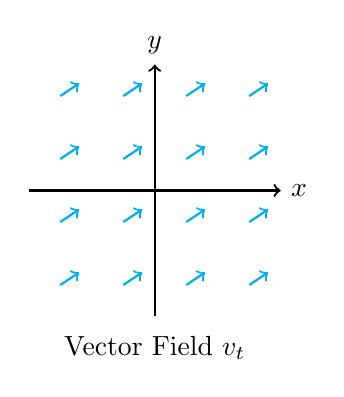
\begin{tikzpicture}[scale=0.8]
            \draw[->, thick] (-2,0) -- (2,0) node[right] {$x$};
            \draw[->, thick] (0,-2) -- (0,2) node[above] {$y$};
            \foreach \x in {-1.5,-0.5,0.5,1.5}
                \foreach \y in {-1.5,-0.5,0.5,1.5}
                    \draw[->, cyan, thick] (\x,\y) -- (\x+0.3,\y+0.2);
            \node at (0,-2.5) {Vector Field $v_t$};
        \end{tikzpicture}
    \end{columns}
\end{frame}

% Section 2: Mathematical Formalism
\section{Mathematical Formalism}

\begin{frame}{The Continuity Equation}
    We want to transform a simple prior distribution $p_0$ (Noise) to a complex data distribution $p_1$ (Data).
    
    A time-dependent vector field $v_t: \R^d \to \R^d$ defines a flow $\phi_t$ via the ODE:
    $$ \frac{d}{dt}\phi_t(x) = v_t(\phi_t(x)) $$
    
    This generates a probability path $p_t$. For mass to be conserved, $p_t$ must satisfy the \textbf{Continuity Equation}:
    $$ \frac{\partial p_t}{\partial t} + \nabla \cdot (p_t v_t) = 0 $$
    
    \textbf{Intuition}: The change in density at a point is equal to the net flow of mass into/out of that point.
\end{frame}

\begin{frame}{The Objective: Matching the Vector Field}
    If we knew the ground truth vector field $u_t$ that generates $p_{data}$, we could just regress it:
    $$ \loss_{FM}(\theta) = \E_{t \sim \mathcal{U}[0,1], x \sim p_t(x)} || v_\theta(x) - u_t(x) ||^2 $$
    
    \textbf{Problem}: 
    \begin{itemize}
        \item We don't know $p_t$ (the intermediate distributions).
        \item We don't know $u_t$ (the vector field).
        \item We only have samples from $p_1$ (Data) and can sample $p_0$ (Noise).
    \end{itemize}
\end{frame}

\begin{frame}{Conditional Flow Matching (CFM)}
    \begin{block}{The Key Insight (Lipman et al., 2023)}
        It is hard to match the aggregate flow, but easy to match a \textbf{conditional} flow.
    \end{block}
    
    We assume the total probability path is a mixture of simple paths conditioned on data $x_1$:
    $$ p_t(x) = \int p_t(x|x_1) q(x_1) dx_1 $$
    
    The \textbf{CFM Theorem} states that minimizing the loss w.r.t. the conditional field $u_t(x|x_1)$ is equivalent to minimizing the global FM loss:
    $$ \nabla_\theta \loss_{FM}(\theta) \approx \nabla_\theta \E_{t, x_1, x_0} [ || v_\theta(x_t, t) - u_t(x_t|x_1) ||^2 ] $$
\end{frame}

\begin{frame}{Defining the Conditional Path}
    We need to choose a path $p_t(x|x_1)$ that goes from noise to $x_1$. 
    We choose the \textbf{Optimal Transport} path (straight line):
    
    $$ x_t = (1 - t)x_0 + t x_1, \quad x_0 \sim \mathcal{N}(0, I) $$
    
    The corresponding unique vector field is:
    $$ u_t(x|x_1) = x_1 - x_0 $$
    
    \textbf{Why this choice?}
    \begin{itemize}
        \item \textbf{Simplicity}: Constant velocity for each pair.
        \item \textbf{Efficiency}: Straight paths imply we can take larger steps during sampling (Euler).
        \item \textbf{Stability}: Regression target is bounded and well-behaved.
    \end{itemize}
\end{frame}

% Section 3: Implementation
\section{Implementation}

\begin{frame}[fragile]{Training Algorithm}
    \begin{enumerate}
        \item Sample data $x_1 \sim p_{data}$ and noise $x_0 \sim \mathcal{N}(0, I)$.
        \item Sample time $t \sim \mathcal{U}[0, 1]$.
        \item Interpolate: $x_t = (1-t)x_0 + t x_1$.
        \item Compute target velocity: $u_t = x_1 - x_0$.
        \item Minimize MSE: $|| v_\theta(x_t, t) - u_t ||^2$.
    \end{enumerate}
\end{frame}

\begin{frame}{Model Architecture: MLP}
    We used a straightforward MLP, but the \textbf{conditioning on time} $t$ is critical.
    
    \textbf{Architecture details}:
    \begin{itemize}
        \item \textbf{Input}: $x \in \R^2$ concatenated with Time Embedding $emb(t) \in \R^{32}$.
        \item \textbf{Backbone}: 3 $\times$ Linear(128) $\to$ SiLU.
        \item \textbf{Output}: $\hat{v} \in \R^2$.
    \end{itemize}
    
    \textbf{Time Embeddings}:
    Standard sinusoidal embeddings (Vaswani et al.) allow the network to distinguish $t=0.1$ (high noise) from $t=0.9$ (fine detail) effectively.
    $$ emb(t)_i = \sin(t \cdot \omega_i) \quad \text{or} \quad \cos(t \cdot \omega_i) $$
\end{frame}

\begin{frame}[fragile]{Sampling: Solving the ODE}
    \begin{columns}
        \column{0.5\textwidth}
        To generate a sample:
        \begin{enumerate}
            \item Sample noise $x_0 \sim \mathcal{N}(0, I)$.
            \item Numerical Integration from $t=0$ to $1$.
        \end{enumerate}
        
        We used \textbf{Euler Method}:
        $$ x_{t+dt} = x_t + v_\theta(x_t, t) \cdot dt $$
        
        Since our paths are straight (thanks to OT), Euler is surprisingly accurate even with few steps (N=20 to 100).
        
        \column{0.5\textwidth}
        \begin{minted}[fontsize=\footnotesize]{python}
# Pseudocode
x = randn(batch_size, 2)
dt = 1 / steps
for i in range(steps):
    t = i / steps
    # Predict velocity
    v = model(x, t)
    # Update state
    x = x + v * dt
return x
        \end{minted}
    \end{columns}
\end{frame}

\section{Results}

\begin{frame}{Qualitative Results}
    \begin{center}
        \includegraphics[width=0.45\textwidth]{imgs/reconstruction_plot.png}
        \caption{Transformation from Noise (Left) to Data (Right)}
    \end{center}
    \begin{itemize}
        \item The model successfully learned the distribution.
        \item Trajectories are straight lines (Optimal Transport).
    \end{itemize}
\end{frame}

\begin{frame}{Vector Field Visualisation}
     \begin{center}
        \includegraphics[width=0.6\textwidth]{imgs/reconstruction_MNIST_.png} 
        \footnote{Note: Assuming this image shows more complex data or vector fields.}
    \end{center}
    The vector field is smooth and points directly towards the data modes.
\end{frame}

\section{Comparison \& Conclusion}

\begin{frame}{Flow Matching vs RealNVP}
    \begin{table}[]
        \begin{tabular}{@{}lll@{}}
            \toprule
            Feature & RealNVP (Discrete Flow) & Flow Matching (Continuous) \\ \midrule
            \textbf{Architecture} & Constrained (Invertible) & Free-form MLP \\
            \textbf{Training} & Exact Likelihood (NLL) & Vector Regression (MSE) \\
            \textbf{Sampling} & 1 pass (Fast) & ODE Solve (Iterative, but fast w/ OT) \\
            \textbf{Expressivity} & Limited by coupling & Universal Approximator \\ \bottomrule
        \end{tabular}
    \end{table}
    \textbf{Conclusion}: Flow Matching creates higher quality samples with simpler training dynamics, at the cost of iterative sampling.
\end{frame}

\begin{frame}
    \centering
    \Huge Thank You!
    \vspace{1cm}
    \large Questions?
\end{frame}

\end{document}
